Poco efficace la pagina 404. Viene semplicemente detto all'utente che c'è stato un errore. Questo approccio presenta i seguenti svantaggi:
\begin{itemize}
	\item Cosa vuol dire 404? L'utente normale non è interessato o non sa cosa sia l'errore 404. perché mostrarlo allora?
	\item Se l'utente è arrivato alla pagina 404 vuol dire che ha copiato male l'indirizzo o arriva da un broken link (magari da una pagina esterna a Caccaro.com). Quindi perché non mostragli subito dei link ai prodotti? In ogni caso la pagina 404 rimane pur sempre un errore, che quasi sicuramente è poco gradito all'utente. Sarebbe meglio mostrare dei messaggi simpatici per far capire il problema all'utente, ma indorando la pillola.
\end{itemize}

\begin{figure}[H]
	\centering
	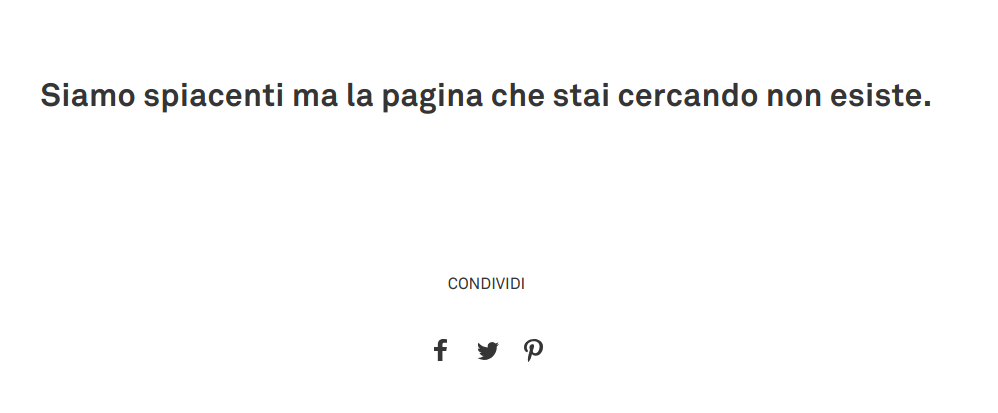
\includegraphics[width=\textwidth ,keepaspectratio]{sez/Varie/img/404.png}
	\caption{Nemmeno il cucchiaio.}
\end{figure}

\begin{center}
\begin{Large}
\textbf{VOTO}\\
\vspace{0.1cm}
\end{Large}
\begin{huge}
5+
\end{huge}
\end{center}